\documentclass{beamer}
%
% Choose how your presentation looks.
%
% For more themes, color themes and font themes, see:
% http://deic.uab.es/~iblanes/beamer_gallery/index_by_theme.html
%
\mode<presentation>
{
  \usetheme{Madrid}      % or try Darmstadt, Madrid, Warsaw, ...
  \usecolortheme{default} % or try albatross, beaver, crane, ...
  \usefonttheme{default}  % or try serif, structurebold, ...
  \setbeamertemplate{navigation symbols}{}
  \setbeamertemplate{caption}[numbered]
} 

\usepackage[norsk, UKenglish]{babel}
%\usepackage[utf8x]{inputenc}

\title[\LaTeX{} for Tekna Student]{\LaTeX{} course for Tekna Student}
\author{Leif Andreas Hirsti}
\institute{Tekna Ung Agder}
\date{\today}

\begin{document}

\begin{frame}
  \titlepage
\end{frame}

% Uncomment these lines for an automatically generated outline.
\begin{frame}{Outline}
  \tableofcontents
\end{frame}


\section{Plan for the day}
\subsection{About me}
\begin{frame}{About me}

\begin{minipage}{0.64\textwidth}
\begin{itemize}
    \item Bachelor's degree in Mechanical engineering at Høgskolen i Oslo og Akershus (Today OsloMet) finished in 2017
    \item Master's degree in Cybernetics at NTNU in 2019
    \item Moved to Kristiansand and started at NOV as Design Engineer in August 2019
    \item Has since November 2021 been working at SLB -- Cameron Sense AS as a Software Engineer
\end{itemize}
\end{minipage}
\hfill
\begin{minipage}{0.29\textwidth}
\begin{figure}

\includegraphics[width=\textwidth]{LAH.png}
\caption{\label{fig:LAH}At a landrig in Saudi-Arabia on 17th of May 2022.}
\end{figure}
\end{minipage}

\end{frame}

\begin{frame}{About me}

\begin{alertblock}{Tekna life}
\begin{itemize}
    \item Tekna member since August 2017, student member in Trondheim
    \item Part of Tekna Ung Agder since January 2020. Doing social events for newly educated members up to the age of 37 years -- \href{https://www.facebook.com/groups/1077086612463991}{Tekna Ung Agder on Facebook}
    \item Leader of Tekna bedriftsgruppe Cameron Sense since January 2023
\end{itemize}
\end{alertblock}

\begin{block}{My \LaTeX{} experience}
\begin{itemize}
    \item Used since my bachelor thesis at HiOA
    \item Used it for all projects and thesis at NTNU
    \item Using \LaTeX{} for CV and cover letters
\end{itemize}
\end{block}

\end{frame}
\subsection{Setup}
\begin{frame}{Setup}

We will go through the following topics using report template. This will include:
\vfill
\begin{minipage}{0.49\textwidth}
\begin{itemize}
    \item General setup
    \begin{itemize}
        \item Documentclass
        \item Packages
        \item Page numbering
        \item Chapter and sections
        \item Table of contents 
        \item Include and input
    \end{itemize}
    \item Equations
    \item Tables
    \item Enumerate
\end{itemize}
\end{minipage}
\hfill
\begin{minipage}{0.49\textwidth}
\begin{itemize}
    \item Itemize
    \item Figures
    \item Drawings
    \item Bibliography
    \item Appendix
    \item Beamer (presentation)
    \item Use of \LaTeX{} in MS word
\end{itemize}
\end{minipage}
\end{frame}

\section{Some \LaTeX{} Examples}
\subsection{Boxes}
\begin{frame}{Boxes}

\begin{itemize}
  \item Your introduction goes here!
  \item Use \texttt{itemize} to organize your main points.
\end{itemize}

\vskip 1cm

\begin{block}{Examples}
Some examples of commonly used commands and features are included, to help you get started.
\end{block}

\begin{alertblock}{Important theorem}
Sample text in red box
\end{alertblock}

\begin{examples}
Sample text in green box. The title of the block is ``Examples".
\end{examples}
\end{frame}
\subsection{Tables and Figures}
\begin{frame}{Tables and Figures}

\begin{itemize}
\item Use \texttt{tabular} for basic tables --- see Table~\ref{tab:widgets}, for example.
\item You can upload a figure (JPEG, PNG or PDF) using the files menu. 
\item To include it in your document, use the \texttt{includegraphics} command (see the comment below in the source code).
\end{itemize}


% Commands to include a figure:
\begin{figure}
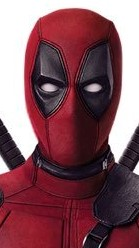
\includegraphics[width=0.1\textwidth]{Deadpool.jpg}
\caption{\label{fig:your-figure}Caption goes here.}
\end{figure}

\begin{table}
\centering
\begin{tabular}{l|r}
Item & Quantity \\\hline
Widgets & 42 \\
Gadgets & 13
\end{tabular}
\caption{\label{tab:widgets}An example table.}
\end{table}

\end{frame}

\subsection{Mathematics}
\begin{frame}{Readable Mathematics}

Let $X_1, X_2, \ldots, X_n$ be a sequence of independent and identically distributed random variables with $\text{E}[X_i] = \mu$ and $\text{Var}[X_i] = \sigma^2 < \infty$, and let
$$S_n = \frac{X_1 + X_2 + \cdots + X_n}{n}
      = \frac{1}{n}\sum_{i}^{n} X_i$$
denote their mean. Then as $n$ approaches infinity, the random variables $\sqrt{n}(S_n - \mu)$ converge in distribution to a normal $\mathcal{N}(0, \sigma^2)$.

\vfill
You can also use \texttt{$\backslash$begin\{align\}}
\begin{align}
    x &= 2x + 3 \\
    y &= 3x - 4
\end{align}
\end{frame}



\end{document}
